\chapter{Project milestones}

What follows are milestones for the project development.
Achieving each one is a step closer to the end goal of a functioning documentation-generating tool.

The basis for said milestones is on the analysis of current documentation tools (see \ref{sec:whatisavailable}), the developer needs (see \ref{sec:whatdouserswant}), personal experience, and general project development guidelines.

\section{Proof of concept}

Creating a proof of concept program will help understand whether the project is realistic, what challenges will occur and how to overcome them.
The main drawback of this is that it will take additional time; however, the gained perspectives are quintessential for the correct planning of the project.

The main focus of this milestone is to find out how to extract the necessary data for documentation generation and attempt to generate said documentation.
All other requirements based on the takeaways from the survey (see \ref{ssec:questionnaireeval}) can be omitted from this stage, as they have been proven via other personal projects or are publicly available for reference.

\section{Evaluations and project planning}

Concise planning of the project, based on the gained experience from the proof of concept, will, as a result, yield a higher quality product.
Extensibility will be the key feature of the project. Careful planning of the code structure is required to avoid unnecessary complications.
Meanwhile, the planning phase shouldn't take unreasonable effort, as the ratio of time spent to results will diminish over time (as seen in \ref{fig:overplanning}). \cite{ruparelia_stop_2016}

\begin{figure}[H]
    \centering
    \caption{Overplanning visualized}
    \label{fig:overplanning}
    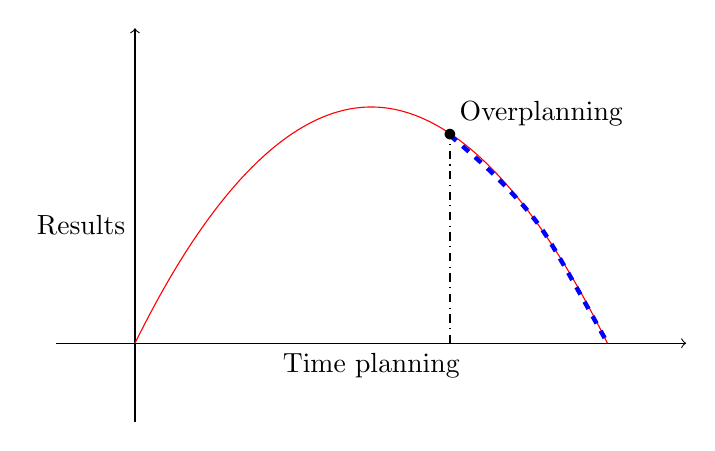
\begin{tikzpicture}
        \draw [->] (-4, 0)--(4,0) node [midway, below]{Time planning};
        \draw [->] (-3, -1)--(-3,4) node[left, midway]{Results};

        \draw [red] (0, 3) parabola(-3,0); % Left
        \draw [red] (0, 3) parabola(3,0); % Right
        \draw [ultra thick, blue, dashed] plot [smooth] coordinates {(1, 2.64) (1.6,2.1) (2.2, 1.40) (3, 0)}; % Right

        \draw [dash dot] (1,0)--(1, 2.64);

        \draw (1, 2.64) node [above right]{Overplanning};
        \draw (1, 2.64) node {$\bullet$};
    \end{tikzpicture}
\end{figure}

\section{Basic structure}

Setting up the project structure and introducing interfaces will pave its foundation. The resulting project structure should cohere with the plan from the previous milestone.

Ensuring minimum coupling of interfaces will be the priority of this milestone, as it will maximize the modularity of the parts composing the project.
Other goals include:
\begin{itemize}
    \item Setting up a \ref{itm:cicd} build environment
    \item Documenting the interfaces
    \item Preparing an empty test console application for the next milestone
\end{itemize}

\section{Processing libraries}

The focus of this milestone will be the creation of working processing libraries that will serve as the core of the application. Said libraries will take some input and generate documentation as an output. The types of libraries and their implementation depend on the previous milestones. The result of this milestone will be a set of working libraries testable via a console application.

\section{GUI application}

The \ref{itm:gui} application will serve as the facade to users utilizing the tool. Said application must be cross-platform, have a modern design, and provide as seamless a user experience as possible, considering the extensible nature of the tool.

\section{Markdown for Git plugin}

Creating the first plugin for the tool will be the final milestone for the time being, as its creation solves the goal of this thesis.
The plugin will be composed of the processing libraries created in the fourth milestone, and necessary UI elements.